\documentclass[10pt]{article}

\usepackage[a4paper, margin=2.6cm]{geometry}
\usepackage{amsmath}
\usepackage{booktabs}
\usepackage{graphicx}
\usepackage{caption}
\usepackage{float}
\usepackage{microtype}
\usepackage[hidelinks]{hyperref}

\graphicspath{{../../plots/}}
\captionsetup{font=small, labelfont=bf}

\newcommand{\Nopt}{N_{\mathrm{opt}}}
\newcommand{\Dopt}{D_{\mathrm{opt}}}
\newcommand{\e}[1]{\times 10^{#1}}

\title{Chinchilla Scaling Laws for Tiny Transformers}
\author{Hyeonseok Jung}
\date{}

\begin{document}
\maketitle

\begin{abstract}
I train transformers ranging from 5K to 3M parameters on 6-digit
multiplication and derive compute-optimal scaling laws for them, following
the three approaches of Hoffmann et al.\ (2022). All three approaches
recover the Chinchilla conclusion that parameters and data should grow in
roughly equal proportion with compute, with fitted exponents between 0.49
and 0.57 for the dense family. A mixture-of-experts family scales its
active parameters at the same rate, and the benefit of sparsity appears in
the constant of the frontier. The main obstacle was grokking. Above a
compute threshold, runs fall discontinuously below every smooth fit. This
behaviour dictated the choice of task, the fitting windows, and the
interpretation of the fitted loss floor.
\end{abstract}

\section{Problem statement}

This report is about teaching small transformers 6-digit multiplication and
deriving Chinchilla scaling laws from the resulting training runs. Following
Hoffmann et al.\ (2022), I assume power-law frontiers
\begin{equation}
  \Nopt(C) \propto C^{a}, \qquad \Dopt(C) \propto C^{b},
\end{equation}
where $C$ is the training compute budget, $N$ the number of parameters, and
$D$ the number of training tokens. I estimate $(a, b)$ with the paper's
three approaches, for a dense model family and for a mixture-of-experts
(MoE) family.

\subsection{Why 6-digit multiplication}

The exercise this report started from proposes up-to-3-digit addition. I
implemented that first and found that it cannot support a scaling analysis.
At the larger step counts and FLOP budgets, every model in the sweep,
including the smallest, saturated the task and reached 100\% accuracy on the
answer digits. Past that point the loss keeps falling, but it no longer
measures ability. Once a model predicts every digit correctly, the remaining
cross-entropy only reflects how much probability the softmax assigns to the
already-correct answer, and it is driven by the sharpening of the logits
over training rather than by anything learned about addition. Loss differences between saturated models therefore do not rank them. The
behaviour below saturation was also unsuitable for fitting. Models sat near the
digit-statistics loss and then \emph{grokked}, jumping to the solution, and
smaller models often jumped before larger ones. Chinchilla's framework
assumes a loss that falls smoothly with compute and that remains a
meaningful measure of ability over the whole measured range, so that a
frontier can be fit through it. I therefore made
the task harder until the still-learning regime filled the compute range I
could afford. With 6-digit multiplication the jump does not appear until
roughly $7\e{14}$ training FLOPs, which leaves about three decades of clean
power-law behaviour. All fits below use that window. The transition itself
is measured in Appendix~\ref{app:grokking}.

\subsection{Task}

Each example is a single 26-token sequence \texttt{lhs*rhs=answer} over a
12-token vocabulary (digits 0--9, \texttt{*}, \texttt{=}). Every number is
zero-padded to a fixed width, so both operands are always exactly 6 digits,
the answer is always exactly 12 digits, and all sequences share one layout.
Loss and accuracy are computed only on the 12 answer digits. Each batch is
sampled uniformly at random from the $10^{12}$ possible operand pairs, and a
run sees at most $10^{9}$ examples, so duplicates are rare and the sampler
never runs out of fresh data. The training loss can therefore be used as the
test loss, which is the same infinite-data assumption as in the paper (their
footnote~2).

\subsection{Models}

The models are pre-RMSNorm decoder-only transformers with grouped-query
attention, QK-norm, RoPE, and SwiGLU MLPs, computed in bf16. The dense
family spans 55 sizes from 4.8K to 3.17M parameters. The MoE family replaces
every MLP with a top-1-of-4-experts layer and covers 13 sizes from 20K to
2.98M \emph{active} parameters. Precise sizings and hyperparameters are
listed in Appendix~\ref{app:zoo}. Appendix~\ref{app:ablations} reports
ablations of RoPE and QK-norm at the largest size.

\subsection{Training}

All models are trained with AdamW at batch size 256. The initial learning
rate is set per model and follows a cosine schedule that decays by a factor
of 10 over the full run. The loss is logged at every step. Two sweep
protocols feed the analysis (Table~\ref{tab:sweeps}).

\begin{table}[h]
\centering
\small
\begin{tabular}{llrr}
\toprule
sweep & protocol & dense & MoE \\
\midrule
fixed-horizon & each size $\times$ horizons of 4k--256k steps & 257 & 52 \\
fixed-budget  & 8 budgets, $C = 1.8\e{13} \dots 3\e{15}$, curated size range per budget & 206 & 67 \\
\midrule
total & & \textbf{463} & \textbf{119} \\
\bottomrule
\end{tabular}
\caption{Training runs feeding the analysis.}
\label{tab:sweeps}
\end{table}

\subsection{Compute accounting}

Instead of the $6ND$ approximation, forward FLOPs per token are computed
exactly for each architecture, including every matmul, normalisation,
activation, and residual addition, and multiplied by 3 to account for the
backward pass (Appendix~\ref{app:flops}). The difference is not negligible at
these scales; the exact count exceeds the $6N$-per-token rule by 17\% for
the smallest model and by 3\% for the largest. All budgets $C$ in this report are training
FLOPs under this accounting.

\section{Approach 1: fix model sizes and vary number of training tokens (dense)}

In the first approach I vary the number of training steps for the fixed
family of model sizes. Each size is trained for four separate horizons of
4k, 8k, 16k, and 32k steps, a range of $8\times$ in seen tokens, and subsets
of the family are trained further at 64k, 128k, and 256k steps to extend the
high-compute end. The cosine schedule decays the
learning rate by a factor of 10 over each horizon, so a longer horizon is a
separate run rather than a continuation. For each run I smooth the loss
curve with a Gaussian filter ($\sigma = 20$ steps) and interpolate it, which
gives a continuous mapping from FLOP count to training loss. At 1{,}500
log-spaced FLOP values I then determine which run achieves the lowest
interpolated loss and record its model size and token count. Finally, I fit
power laws through these points to estimate the optimal model size and token
count for any budget (Figure~\ref{fig:a1}).

\begin{figure}[h]
\centering
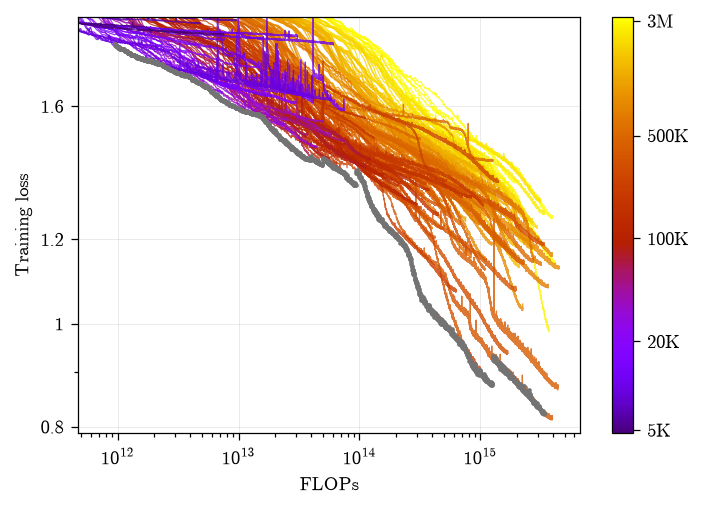
\includegraphics[width=0.365\textwidth]{dense/a1_envelope.png}\hfill
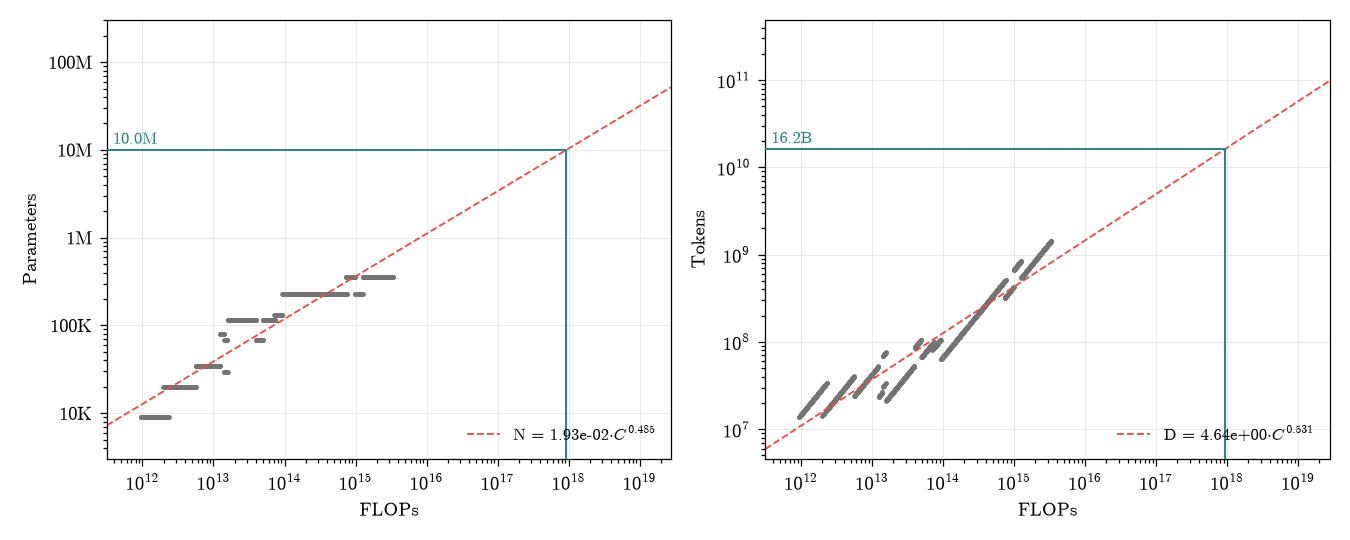
\includegraphics[width=0.62\textwidth]{dense/a1_frontier.png}
\caption{Approach 1. Left: training curves coloured by model size; grey
points mark the lower envelope. Centre and right: model size and token count
of the envelope, with power-law fits. The teal projection marks where the
fit predicts a 10M-parameter model becomes compute-optimal, at
$C \approx 9.3\e{17}$ FLOPs and 16.2B tokens.}
\label{fig:a1}
\end{figure}

The training curves in Chinchilla are smooth enough that the raw envelope
can be used directly. Mine are noisier, so I truncate the envelope where fewer than 10 distinct model
sizes still reach the budget, which cuts the fit at $C = 3.4\e{15}$. Past
that point a budget is won by whichever run happens to be the only one
there, and those lone winners are worse per FLOP than the frontier at
smaller budgets. One validity check from the paper also fails and should be noted as a caveat. Chinchilla report that every envelope point comes from the
final 15\% of a run (their footnote~4). In my data only 17.6\% do, 62\% come
from the final half, and the median winning point sits at 60\% of its run.
This suggests that at this scale the envelope is won mid-run much more
often than in their setting.

The fitted frontier is
\begin{equation}
  \Nopt = 1.93\e{-2}\, C^{0.485}, \qquad
  \Dopt = 4.64\, C^{0.531}.
\end{equation}

\section{Approach 2: IsoFLOP profiles (dense)}

In the second approach I fix eight training FLOP budgets from $1.8\e{13}$ to
$3\e{15}$ and, for each budget, train a curated range of model sizes exactly
to that budget. The number of steps for each model follows from the budget
and its per-token cost, and the cosine schedule is set to match that
horizon. For each budget I fit the final smoothed loss against $\log N$ with
a parabola and take the vertex as $\Nopt$; $\Dopt$ follows from the budget.
A power law through the vertices gives the frontier (Figure~\ref{fig:a2}).

I deviate from the paper in two ways. First, I reject grokked runs before
fitting. For each budget I fit the parabola to all points by least squares
and compute the standard deviation $\sigma$ of its residuals. Runs whose
loss sits more than $2\sigma$ below the fitted curve are dropped and the
parabola is refit, for at most three iterations and never below four
remaining points. The rejection is one-sided because the two
kinds of outlier have different causes. A run below the bulk is one that already grokked, and it
would drag the vertex toward itself; a run above the curve is an ordinary
under-trained model and is legitimate data. In practice the rule removes
between zero and four runs per budget out of 12 to 24, so its effect is limited to
removing the grokked tail. Second, I exclude two
budgets before fitting. At $C = 3\e{14}$ the fitted vertex lands at the far-left edge of
the sampled model range, which means the minimum was not actually located.
At $C = 1.8\e{15}$ the fitted parabola is concave and has no minimum at all.
Six budgets remain (Table~\ref{tab:a2dense}).

\begin{figure}[h]
\centering
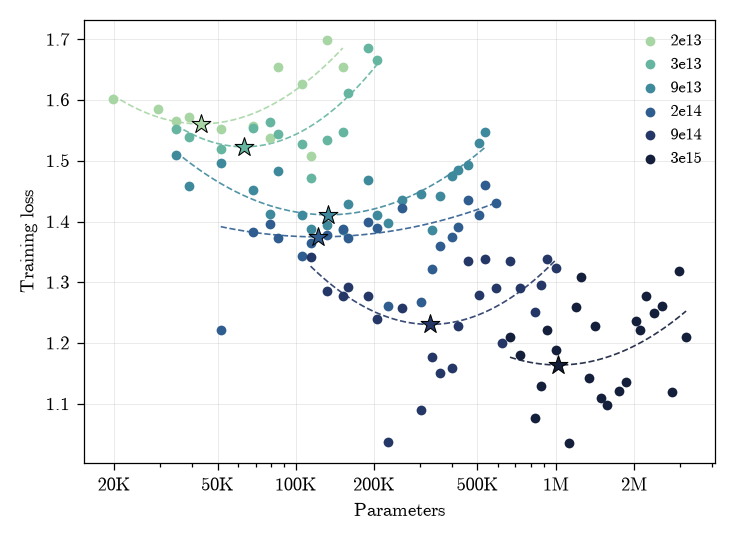
\includegraphics[width=0.35\textwidth]{dense/a2_isoflop.png}\hfill
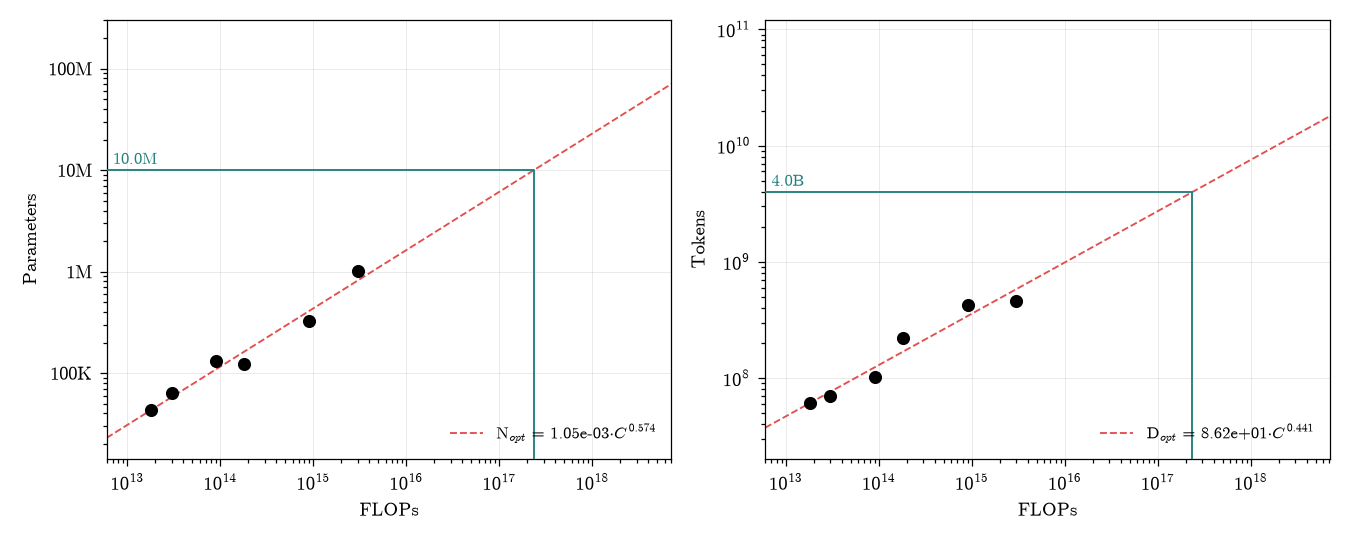
\includegraphics[width=0.63\textwidth]{dense/a2_frontier.png}
\caption{Approach 2. Left: isoFLOP profiles; $\star$ marks each fitted
optimum. Centre and right: the frontier through the vertices. The
10M-parameter projection from this fit is $C \approx 2.4\e{17}$ FLOPs and
4.0B tokens.}
\label{fig:a2}
\end{figure}

\begin{table}[h]
\centering
\small
\begin{tabular}{rrrrr}
\toprule
$C$ (train FLOPs) & runs & $\Nopt$ & $\Dopt$ & curvature \\
\midrule
$1.8\e{13}$ & 12 & 43.0K & $6.1\e{7}$ & 0.079 \\
$3\e{13}$   & 13 & 63.3K & $7.0\e{7}$ & 0.098 \\
$9\e{13}$   & 23 & 132.8K & $1.0\e{8}$ & 0.057 \\
$1.8\e{14}$ & 22 & 121.8K & $2.2\e{8}$ & 0.023 \\
$9\e{14}$   & 24 & 328.4K & $4.2\e{8}$ & 0.086 \\
$3\e{15}$   & 23 & 1.0M  & $4.6\e{8}$ & 0.069 \\
\bottomrule
\end{tabular}
\caption{Per-budget isoFLOP fits for the dense family, after the window
filter and exclusions.}
\label{tab:a2dense}
\end{table}

The fitted frontier is
\begin{equation}
  \Nopt = 1.05\e{-3}\, C^{0.574}, \qquad
  \Dopt = 86.2\, C^{0.441}.
\end{equation}

\section{Approach 3: fitting a parametric loss function (dense)}

In the third approach I fit every run's final smoothed loss with the risk
decomposition proposed in the paper,
\begin{equation}
  \hat L(N, D) = E + \frac{A}{N^{\alpha}} + \frac{B}{D^{\beta}},
\end{equation}
minimising a Huber loss ($\delta = 10^{-3}$) on the log-residuals with
L-BFGS and selecting the best fit from a grid of initialisations. This is
the paper's estimator, unchanged. The closed form of the constrained optimum
gives $a = \beta/(\alpha+\beta)$ and $b = \alpha/(\alpha+\beta)$.

I fit only the runs with $C \le 6.6\e{14}$, which keeps 306 of the 463. The
smooth surface model is false above the grokking transition, which
Appendix~\ref{app:grokking} locates at roughly $7\e{14}$.

The fitted parameters are
\begin{equation}
  E = 1.116, \quad A = 30.1, \quad B = 2433, \quad
  \alpha = 0.455, \quad \beta = 0.522
  \;\;\Rightarrow\;\; a = 0.534, \; b = 0.466.
\end{equation}
The 10M-parameter projection from this fit is $C \approx 4.9\e{17}$ FLOPs
and 7.5B tokens.

\begin{figure}[h]
\centering
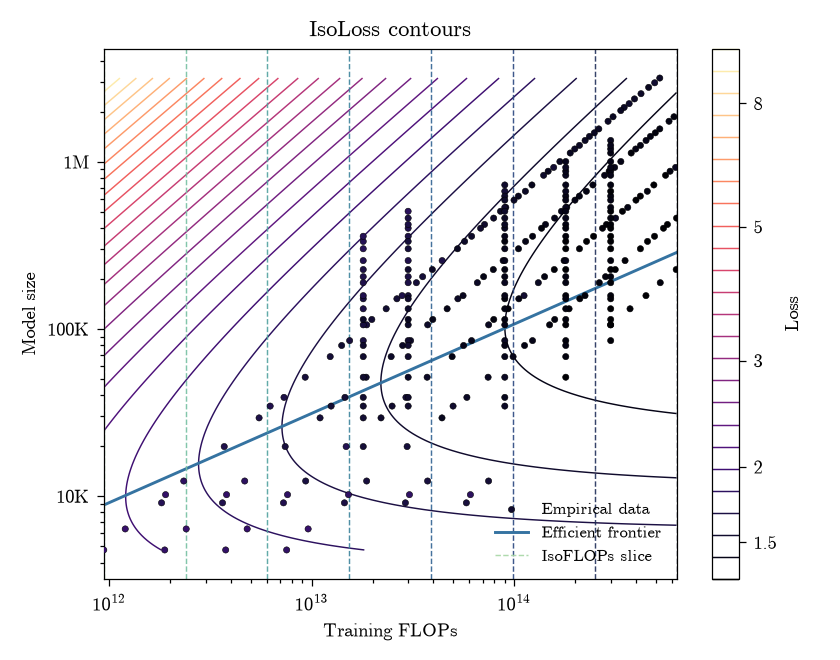
\includegraphics[width=0.49\textwidth]{dense/a3_isoloss_contours.png}\hfill
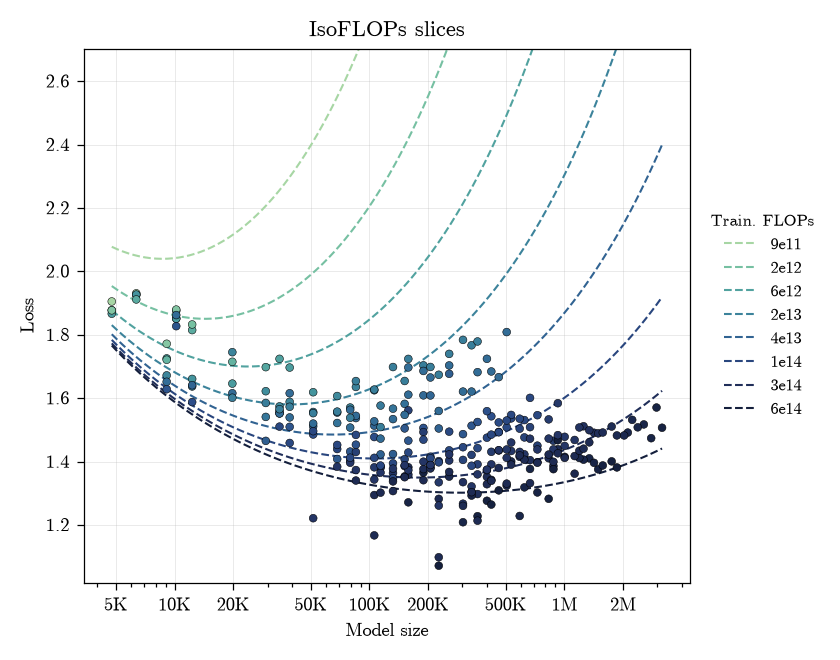
\includegraphics[width=0.49\textwidth]{dense/a3_isoflop_slices.png}
\caption{The parametric fit. Left: isoloss contours with the closed-form
efficient frontier. Right: isoFLOP slices over the raw runs.}
\label{fig:a3}
\end{figure}

The fitted value of $E$ requires some interpretation. In Chinchilla, $E$ is the
entropy of natural text and is a real floor. This task is deterministic, so
its true entropy is zero. The fitted $E \approx 1.12$ is instead the level
that pre-grokking learning converges to; it is the loss the surface predicts
in the limit of unlimited model size and data. Random guessing over the ten
digits costs $\ln 10 \approx 2.30$ nats per answer digit, so this level
corresponds to capturing roughly half of the answer entropy. That half is
the part of the product that can be predicted without the full algorithm,
for example the non-uniform digit statistics of products and the trailing
digits, which depend only on the trailing digits of the operands. Grokked runs
fall below $E$, which is why the surface cannot describe them and why the
compute cut is needed. The fitted law is therefore a scaling law
for this partial-structure phase; it describes how efficiently models learn
the predictable part of the task, and it does not predict when the jump to
the full algorithm occurs.

\section{Dense results}

\begin{table}[h]
\centering
\small
\begin{tabular}{lcc}
\toprule
approach & $a$ \;($\Nopt \propto C^{a}$) & $b$ \;($\Dopt \propto C^{b}$) \\
\midrule
1. Minimum over training curves & 0.485 & 0.531 \\
2. IsoFLOP profiles             & 0.574 & 0.441 \\
3. Parametric fit of the loss   & 0.534 & 0.466 \\
\midrule
Chinchilla (paper)     & 0.50 / 0.49 / 0.46 & 0.50 / 0.51 / 0.54 \\
Kaplan et al.\ (2020)  & 0.73 & 0.27 \\
\bottomrule
\end{tabular}
\caption{Dense scaling exponents against the reference values.}
\label{tab:dense}
\end{table}

All three estimates lie between 0.48 and 0.58, close to equal scaling and
far from the allocation of Kaplan et al.\ (2020). Their fit scales the
model much faster than the data ($a = 0.73$ against $b = 0.27$); under it, a
$10\times$ increase in compute grows the model $5.5\times$ but the data only
$1.8\times$. The spread between approaches is larger than in the paper.
This is expected, since the fits here rest on 582 small and noisy runs,
while theirs used over 400 much smoother ones.

\begin{table}[H]
\centering
\small
\begin{tabular}{lccc}
\toprule
target $N$ & A1: $C$ / $D$ & A2: $C$ / $D$ & A3: $C$ / $D$ \\
\midrule
100K & $7.0\e{13}$ / 104M & $7.8\e{13}$ / 116M & --- \\
1M   & $8.1\e{15}$ / 1.3B & $4.3\e{15}$ / 678M & --- \\
\textbf{10M} & $\mathbf{9.3\e{17}}$ / \textbf{16.2B} & $\mathbf{2.4\e{17}}$ / \textbf{4.0B} & $\mathbf{4.9\e{17}}$ / \textbf{7.5B} \\
\bottomrule
\end{tabular}
\caption{Projected compute-optimal allocations. The $4\times$ spread at 10M
reflects the uncertainty of extrapolating two decades beyond the data;
Chinchilla faced a similar spread when choosing between 40B and 70B
parameters for their validation model.}
\label{tab:proj}
\end{table}

\section{Mixture of experts}

I repeat the three approaches on the MoE family with the same estimators
and the same cuts unless noted. The family has 119 runs over 13 sizes with
top-1-of-4 experts. It covers a 1-in-4 subset of the dense sizes rather
than all 55, because the expert dispatch makes MoE steps slower at these
scales and a full sweep would have taken considerably more
wall-clock time. Every fit is
reported against two parameter counts.
\emph{Active} parameters count only the routed expert and match the dense
family's $N$ and FLOPs per token. \emph{Total} parameters count all four
experts.

\subsection{Approach 1}

The envelope method needs many model sizes competing at every budget, and
the censoring rule of Section~2 drops any budget reached by fewer than 10 of
them. With 13 sizes and four horizons, budgets above $C = 2.2\e{14}$ are
reached by fewer than 10 sizes, so the fixed-horizon runs alone support an
envelope of less than two decades of compute, which is too short to fit a
slope reliably. I therefore include the runs from approach 2 in the
approach-1 analysis, so the 67 fixed-budget runs contribute their training
curves to the same minimum alongside the 52 fixed-horizon runs. This
extends the envelope to $3.0\e{15}$. The cost is that an included run often
wins a budget in the middle of its training rather than near the end, so
only 20.8\% of envelope points come from the last 15\% of a run.
\begin{equation}
  \text{active:} \quad \Nopt = 1.48\e{-4}\, C^{0.639}, \qquad
  \Dopt = 552\, C^{0.380}.
\end{equation}
The steep 0.64 should be interpreted with caution. With 13 sizes the envelope is a
staircase with roughly 5 steps, and the slope is dominated by the largest
jump. Approaches 2 and 3 give more reliable estimates
for the MoE family.

\subsection{Approach 2}

Two budgets are excluded for the same edge-minimum failure as the dense
$3\e{14}$, namely $C = 9\e{14}$ and $1.8\e{15}$. Six budgets remain.
\begin{equation}
  \text{active:} \quad \Nopt = 2.56\e{-3}\, C^{0.536}, \quad
  \Dopt = 35.0\, C^{0.480}; \qquad
  \text{total:} \quad \Nopt \propto C^{0.540}.
\end{equation}

\begin{figure}[h]
\centering

\includegraphics[width=0.5\textwidth]{moe/active_params/a2_isoflop.png}
\caption{MoE isoFLOP profiles, plotted against active parameters.}
\label{fig:moea2}
\end{figure}

\subsection{Approach 3}

The fit uses the same $C \le 6.6\e{14}$ cut and keeps 80 runs.
\begin{align}
  \text{active:} \quad
  & E = 1.139, \; A = 51.9, \; B = 2298, \;
    \alpha = 0.538, \; \beta = 0.515
    \;\Rightarrow\; a = 0.489; \\
  \text{total:} \quad
  & E = 1.137, \; A = 81.6, \; B = 2231, \;
    \alpha = 0.523, \; \beta = 0.513
    \;\Rightarrow\; a = 0.495.
\end{align}

\begin{table}[h]
\centering
\small
\begin{tabular}{lccc}
\toprule
approach & $a$ (active) & $b$ (active) & $a$ (total) \\
\midrule
1. Minimum over training curves & 0.639 & 0.381 & 0.641 \\
2. IsoFLOP profiles             & 0.536 & 0.480 & 0.540 \\
3. Parametric fit of the loss   & 0.489 & 0.511 & 0.495 \\
\bottomrule
\end{tabular}
\caption{MoE scaling exponents.}
\label{tab:moe}
\end{table}

\section{Discussion}

All three approaches, applied to both model families, give similar estimates
of the optimal allocation. Parameter count and training tokens should be
scaled in roughly equal proportions, with fitted exponents between 0.49 and
0.57 for the dense family. This matches the conclusion of Hoffmann et al.\
(2022) despite the much smaller scale and the change of task.

The MoE results suggest that sparsity does not change this allocation. By
approaches 2 and 3, the MoE frontier has the same exponent as the dense
frontier, whether measured in active or in total parameters, and the
difference between the families appears in the constant instead. At a given
budget the optimal MoE model tracks the dense optimum in active parameters,
holds about 3.2 times more total parameters, and reaches a slightly lower
loss (0.97 against roughly 1.16 at $C = 3\e{15}$).

This comparison should be interpreted with some care. The budgets where the
MoE advantage is largest are also the budgets where grokking is most
frequent. Above roughly $7\e{14}$ FLOPs, 24 to 31\% of MoE runs per compute
bin fall more than $3\sigma$ below the smooth surface, compared to 6 to
13\% of dense runs (Appendix~\ref{app:grokking}). Some of the MoE advantage
at these budgets therefore comes from runs that have left the regime the
fitted law describes. The higher transition rate may itself be an effect of
the additional total capacity, but I did not investigate this further.

Finally, the fragile part of this analysis was not the allocation estimate
but the assumptions behind it. The loss needs to fall smoothly with compute
and to remain a meaningful measure of ability over the measured range, and
on arithmetic tasks neither can be taken for granted. The fitted $E$ is the
floor of the pre-grokking phase rather than the entropy of the data, and
the fitted surface does not indicate where the transition will occur. In
this setting, most of the work of deriving the scaling law went into
choosing a task on which its assumptions hold.

\clearpage
\appendix

\section{The grokking transition}
\label{app:grokking}

I fit the approach-3 surface on the runs below $C = 3\e{14}$ only and
measure every run's residual against it. A run more than $3\sigma$ below the
surface has left the smooth regime, and I call it transitioned. I report the
rate of transitioned runs per compute bin rather than the first crossing,
because the dense family has about $4\times$ more runs and would always
produce the earliest grokked run by sampling alone.

\begin{figure}[h]
\centering
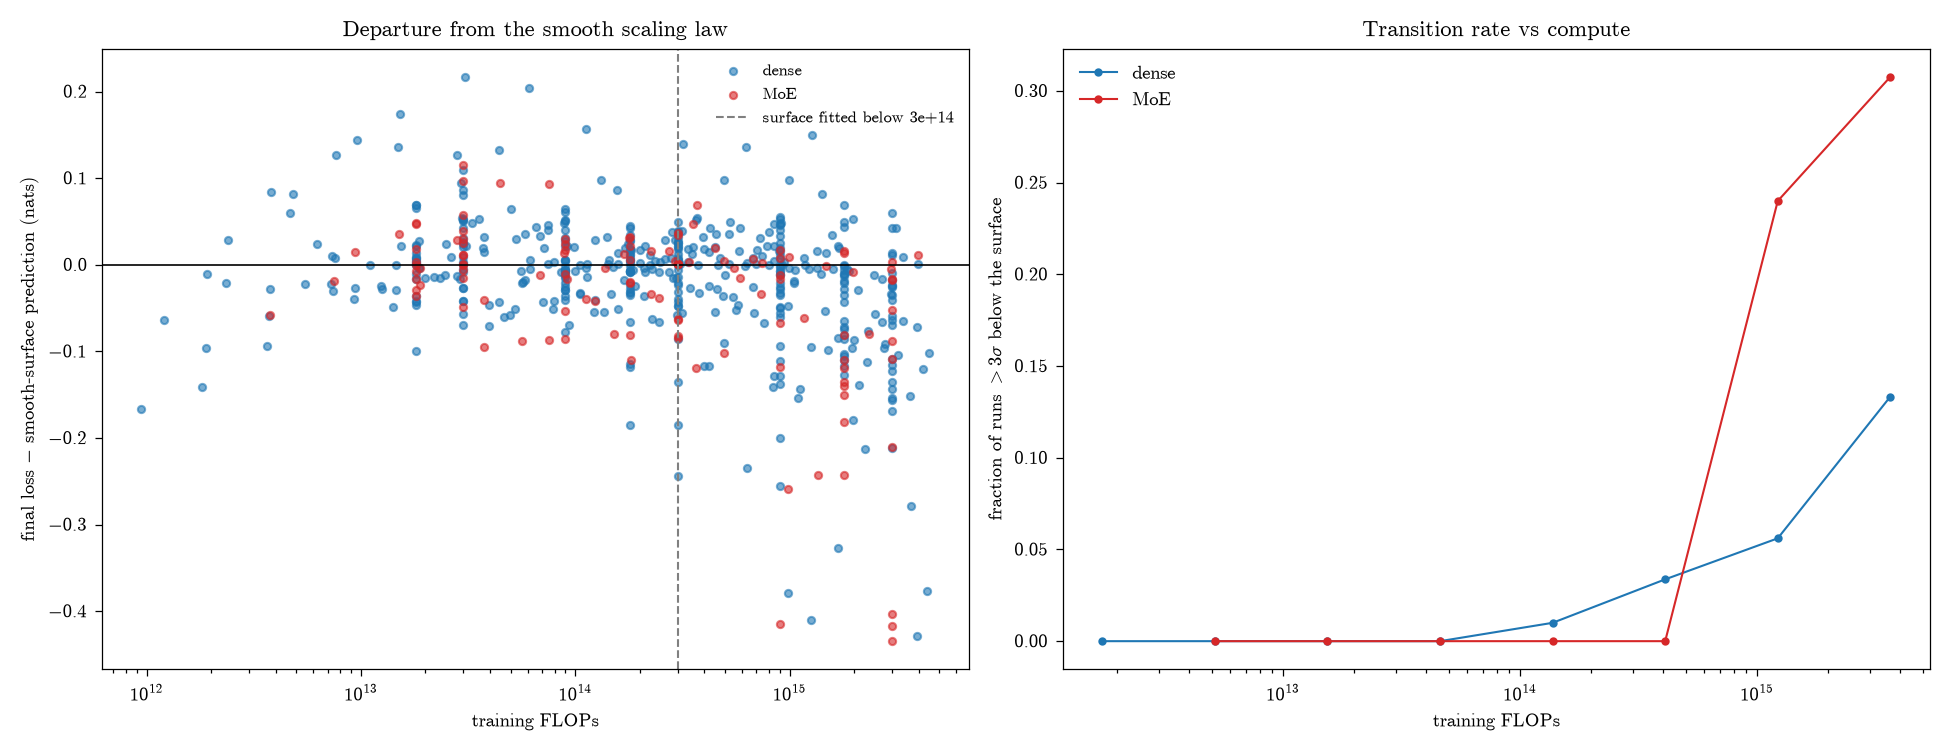
\includegraphics[width=\textwidth]{01_transition.png}
\caption{Left: residuals against the smooth surface fitted below
$3\e{14}$. Right: fraction of runs more than $3\sigma$ below the surface,
per compute bin.}
\label{fig:transition}
\end{figure}

\begin{table}[h]
\centering
\small
\begin{tabular}{lcccc}
\toprule
compute bin & dense runs & dense rate & MoE runs & MoE rate \\
\midrule
$7.9\e{13}$--$2.4\e{14}$ & 100 & 1\%  & 23 & 0\% \\
$2.4\e{14}$--$7.1\e{14}$ & 89  & 3\%  & 22 & 0\% \\
$7.1\e{14}$--$2.1\e{15}$ & 107 & 6\%  & 25 & 24\% \\
$2.1\e{15}$--$6.3\e{15}$ & 45  & 13\% & 13 & 31\% \\
\bottomrule
\end{tabular}
\caption{Transition rates. Bins below $7.9\e{13}$ are 0\% everywhere. The
fitted surfaces are $E{=}1.119$, $\alpha{=}0.442$, $\beta{=}0.536$,
$\sigma{=}0.055$ on 264 dense runs and $E{=}1.127$, $\alpha{=}0.530$,
$\beta{=}0.478$, $\sigma{=}0.047$ on 71 MoE runs.}
\label{tab:transition}
\end{table}

The onset sits at roughly $7\e{14}$ for both families, and the approach-3
cut of $6.6\e{14}$ is chosen just below it. The largest residuals reach
$-0.44$ nats, far larger than the residual noise of the fits
($\sigma \approx 0.05$). Small models sometimes grok ahead of
larger ones, which also roughens the approach-1 envelope at high compute,
where an early-grokking small model can briefly hold the minimum against
every larger size. These measurements are for 6-digit
multiplication; with 3-digit addition the transition happens so early that
no smooth window exists at all, which is why the task was changed.

Figure~\ref{fig:cut} shows how this choice of cut affects the approach-3
result. I refit the surface using only the runs below a threshold and plot
the fitted exponent $a$ against that threshold. Below roughly $3\e{14}$ the
estimates are high and unstable, since few runs remain and they cover a
narrow compute range. Around the chosen cut the dense exponent is stable
near 0.53, and the MoE exponent lies between 0.46 and 0.51, moving by a few
hundredths between nearby thresholds because of its smaller run count. As
the threshold moves past the transition and grokked runs enter the fit,
both exponents fall, to 0.43 for dense and 0.21 for MoE on the full data.
The MoE fit degrades more because a larger fraction of its high-compute
runs have transitioned.

\begin{figure}[H]
\centering
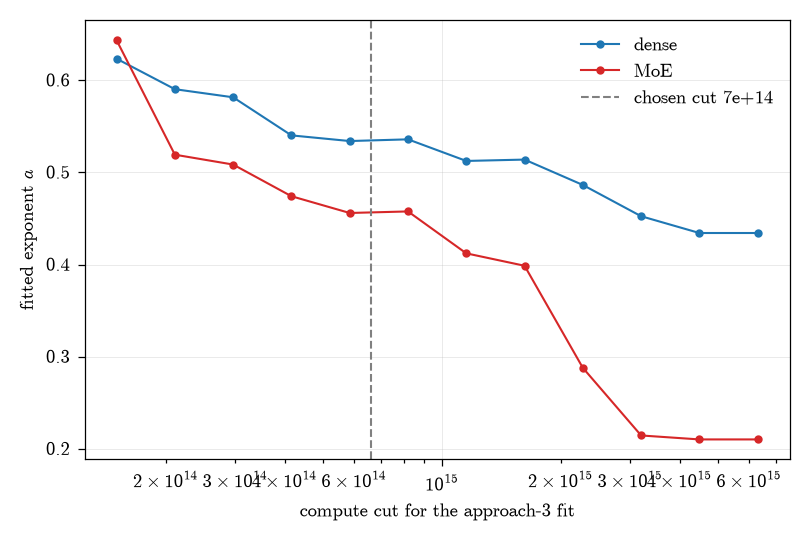
\includegraphics[width=0.62\textwidth]{02_cut_sensitivity.png}
\caption{The fitted exponent $a$ of the approach-3 surface as a function of
the compute cut. Each point refits the surface on the runs below that
threshold. The dashed line marks the cut used in this report.}
\label{fig:cut}
\end{figure}

\clearpage
\section{Architecture ablations}
\label{app:ablations}

The model family fixes two attention details that the main sweeps never
vary: RoPE for position information and QK-norm. To check how much these
choices matter, I trained the largest dense model (3.17M parameters) under
four variants, one per chip of a TPU v5e-4. The baseline keeps RoPE and
QK-norm. The other three variants replace RoPE with a learned absolute
position embedding, remove position information entirely (NoPE), and keep
RoPE but remove QK-norm. Every other setting matches the main runs,
including the seed. Each variant trains for 128,000 steps, four times the
longest horizon the 3.17M model sees in the main sweeps, reaching
$C = 1.7\e{16}$.

\begin{figure}[H]
\centering
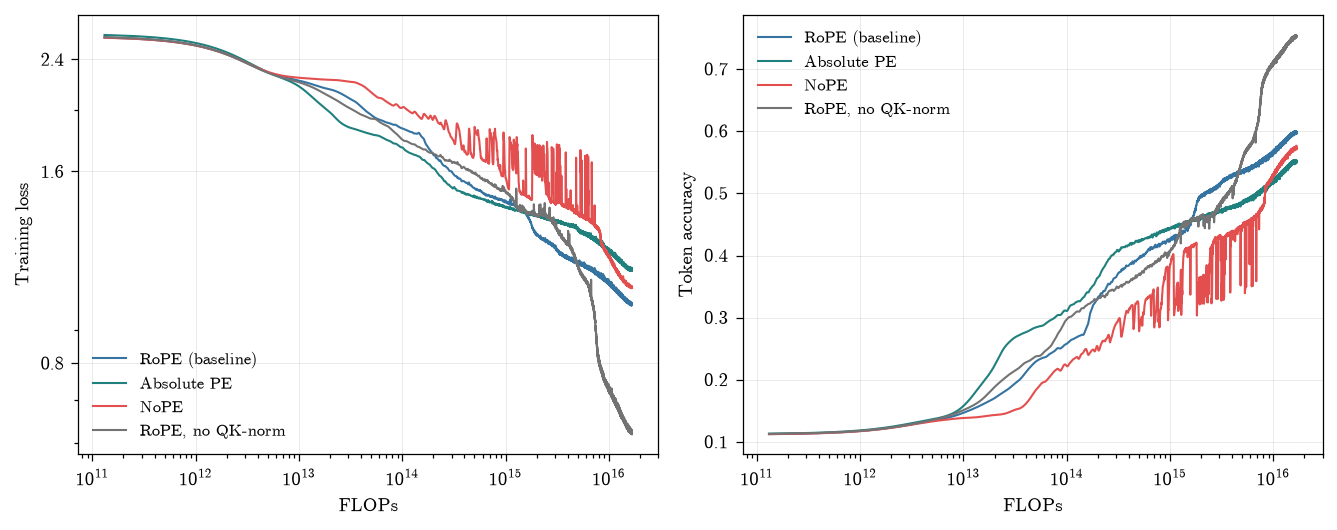
\includegraphics[width=\textwidth]{03_ablations.png}
\caption{Training loss (left) and token accuracy over the 12 answer digits
(right) for four variants of the 3.17M model, each trained for 128,000
steps. Curves are smoothed with the same Gaussian filter as the main
analysis ($\sigma = 20$ steps).}
\label{fig:ablations}
\end{figure}

Figure~\ref{fig:ablations} shows the result. In the smooth regime the
variants behave similarly. At $C = 1\e{15}$ the four losses lie between
1.40 and 1.56. NoPE is consistently the highest and is the only variant
that shows instability, in the form of repeated loss spikes concentrated
between roughly $1\e{15}$ and $7\e{15}$ FLOPs. The variants separate at the
transition. The run without QK-norm transitions first: its loss crosses 1.0
at $C = 6.9\e{15}$ and falls to 0.62 by the end of training, with token
accuracy reaching 75\%. The same run is not fully stable. It shows small
loss spikes between roughly $1\e{15}$ and $7\e{15}$ FLOPs, much lower in
height than the NoPE spikes and absent from the other two variants. The
baseline crosses 1.0 at $1.5\e{16}$, close to
the end of its horizon. This is consistent with the main sweeps, where the
3.17M model had not transitioned by $4.2\e{15}$. Neither position-embedding
replacement transitions within the horizon. Absolute position embeddings
end at a loss of 1.12, matching the fitted floor $E$, and NoPE ends at
1.05. Exact-match accuracy over the full product stays below 1\% for every
variant, so even the transitioned runs remain far from solving the task at
this compute.

Two observations seem worth stating. First, these
architecture choices matter here mainly through the timing of the
transition rather than through the smooth regime, where the four curves
differ by at most about 0.2 nats. Second, removing QK-norm brings the
transition forward by about a factor of 2 in compute. The transition
threshold of Appendix~\ref{app:grokking} is therefore specific to this
architecture, and a different baseline could move it.

\clearpage
\section{FLOP computation}
\label{app:flops}

As in Appendix~F of the paper, I include all operations in the forward pass
and count a multiply-accumulate as 2 FLOPs. Unlike the generic rule, I also
count normalisations, activations, and residual additions, which are not
negligible at these sizes. With $S = 26$ (\texttt{seq\_len}), $V = 12$
(\texttt{vocab\_size}), $D$ (\texttt{d\_model}), $F$ (\texttt{d\_ffw}),
$L$ (\texttt{n\_layers}), $N_q$ query heads, $N_{kv}$ key/value heads, and
$H = 8$ (\texttt{d\_head}):

\begin{itemize}
  \item Embeddings: $2SVD$
  \item Attention (single layer):
  \begin{itemize}
    \item Q, K, V projections: $2SDH(N_q + 2N_{kv})$
    \item QK-RMSNorm and RoPE: $4SN_qH + 4SN_{kv}H + 3S(N_q{+}N_{kv})H + 3SH$
    \item key @ query logits: $2S^2 H N_q$
    \item scaling and softmax: $S^2 N_q + 5 N_q S^2$
    \item softmax @ value reductions: $2S^2 H N_q$
    \item output projection: $2S(HN_q)D$
  \end{itemize}
  \item SwiGLU dense block (single layer, 3 matmuls): $6SDF + 6SF$
  \item Pre-attention and pre-MLP RMSNorm: $2 \times 4SD$; residual additions: $2SD$
  \item Final RMSNorm: $4SD$; final logits: $2SVD$
\end{itemize}
\begin{equation}
  F_{\mathrm{fwd}} = 2SVD + L\,(\mathrm{attn} + \mathrm{mlp} + 10SD) + 4SD + 2SVD,
  \qquad
  \text{FLOPs/token} = F_{\mathrm{fwd}} / S,
\end{equation}
with backward $\approx 2\times$ forward, so training FLOPs per token are
$3 \times F_{\mathrm{fwd}}/S$. As in the paper, the difference against the
$C = 6ND$ rule is small and shrinks with scale; their Table~A4 approaches
1.0 for billion-parameter models. Table~\ref{tab:flops} shows the small
end of the same trend. The ratio is driven by the $O(S^2)$ attention terms,
the embeddings, and the normalisation being relatively larger in small
models.

\begin{table}[h]
\centering
\small
\begin{tabular}{rc}
\toprule
params & FLOPs/token $/\, 6N$ \\
\midrule
19.8K  & 1.17 \\
105.9K & 1.11 \\
533.7K & 1.07 \\
3.17M  & 1.03 \\
\bottomrule
\end{tabular}
\caption{The exact per-token count against the $6N$ rule.}
\label{tab:flops}
\end{table}

\clearpage
\section{Fitting details and exclusions}
\label{app:fitting}

\begin{itemize}
  \item \textbf{Smoothing.} A Gaussian filter with $\sigma = 20$ steps is
    applied to every loss curve before any use.
  \item \textbf{Envelope censoring (approach 1).} Grid points where fewer
    than 10 distinct sizes reach the budget are dropped. Dense keeps
    $C \le 3.4\e{15}$ and MoE keeps $C \le 3.0\e{15}$.
  \item \textbf{Trim fit (approach 2).} The parabola is refit iteratively
    while dropping points more than $2\sigma$ below the curve, for at most 3
    iterations and never below 4 points. The rejection is one-sided because
    grokking only ever lowers loss.
  \item \textbf{Per-budget model windows (approach 2, dense).} Each budget
    fits only the sizes inside a hand-curated window
    (Appendix~\ref{app:budgets}) so that every parabola brackets its
    minimum. 117 of 153 remaining runs pass the windows.
  \item \textbf{Excluded budgets.} Dense $3\e{14}$ (vertex at the range
    edge), dense $1.8\e{15}$ (concave), MoE $9\e{14}$ and $1.8\e{15}$
    (vertex at the range edge).
  \item \textbf{Approach-3 cut.} $C \le 6.6\e{14}$, from
    Appendix~\ref{app:grokking}.
  \item Bootstrap confidence intervals on $(a, b)$, as in Table~2 of the
    paper, are not computed. They would strengthen the exponent tables.
\end{itemize}

\clearpage
\section{Model ranges per FLOP budget}
\label{app:budgets}

\begin{table}[H]
\centering
\small
\begin{tabular}{lll}
\toprule
$C$ (train FLOPs) & dense window ($N$) & MoE range (active $N$) \\
\midrule
$1.8\e{13}$ & 19.8K--151.6K & 4.8K--132.9K \\
$3\e{13}$   & 34.6K--205.5K & 4.8K--206.5K \\
$9\e{13}$   & 34.6K--533.7K & 51.8K--535.8K \\
$1.8\e{14}$ & 51.5K--590.1K & 51.8K--535.8K \\
$3\e{14}$   & 85.2K--727.3K\,$^\dagger$ & 20.0K--729.6K \\
$9\e{14}$   & 114.0K--1.00M & 159.3K--1.01M\,$^\dagger$ \\
$1.8\e{15}$ & 506.1K--2.03M\,$^\dagger$ & 106.5K--2.0M\,$^\dagger$ \\
$3\e{15}$   & 666.7K--3.17M & 257.7K--3.0M \\
\bottomrule
\end{tabular}
\caption{Model sizes entering each isoFLOP fit. $^\dagger$ marks budgets
excluded from the frontier fit, for the reasons in
Appendix~\ref{app:fitting}.}
\label{tab:budgets}
\end{table}

\clearpage
\section{Model zoo}
\label{app:zoo}

All models use $d_{\mathrm{ffw}} = 4\,d_{\mathrm{model}}$,
$d_{\mathrm{head}} = 8$, and $n_{\mathrm{heads}} = n_{kv} =
d_{\mathrm{model}} / 8$. FLOPs/token is the exact forward count of
Appendix~\ref{app:flops}. MoE models share the dense backbone with 4 experts
per MLP and top-1 routing. The initial learning rate of each size was
selected from three options, 1e-2, 3e-3, and 1e-3, by running a short
training run with each and keeping the one with the lowest loss.

\begin{table}[h]
\centering
\footnotesize
\begin{tabular}{rrrrr}
\toprule
params & $L$ & $d_{\mathrm{model}}$ & LR & FLOPs/token \\
\midrule
4.76K & 1 & 16 & 1e-2 & 11{,}792 \\
6.36K & 1 & 16 & 1e-2 & 15{,}056 \\
9.12K & 2 & 16 & 1e-2 & 22{,}752 \\
10.2K & 1 & 24 & 1e-2 & 23{,}820 \\
12.3K & 2 & 16 & 1e-2 & 29{,}280 \\
19.8K & 2 & 24 & 1e-2 & 46{,}392 \\
29.4K & 3 & 24 & 1e-2 & 68{,}964 \\
34.6K & 2 & 32 & 1e-2 & 78{,}224 \\
39.0K & 4 & 24 & 1e-2 & 91{,}536 \\
51.5K & 3 & 32 & 1e-2 & 116{,}504 \\
68.3K & 4 & 32 & 1e-2 & 154{,}784 \\
79.7K & 3 & 40 & 1e-2 & 176{,}332 \\
85.2K & 5 & 32 & 1e-2 & 193{,}064 \\
105.9K & 4 & 40 & 1e-2 & 234{,}416 \\
114.0K & 3 & 48 & 1e-2 & 248{,}448 \\
132.1K & 5 & 40 & 1e-2 & 292{,}500 \\
151.6K & 4 & 48 & 1e-2 & 330{,}432 \\
158.3K & 6 & 40 & 1e-2 & 350{,}584 \\
189.2K & 5 & 48 & 1e-2 & 412{,}416 \\
205.5K & 4 & 56 & 1e-2 & 442{,}832 \\
226.8K & 6 & 48 & 1e-2 & 494{,}400 \\
256.6K & 5 & 56 & 1e-2 & 552{,}812 \\
302.0K & 8 & 48 & 3e-3 & 658{,}368 \\
334.2K & 5 & 64 & 3e-3 & 713{,}688 \\
358.6K & 7 & 56 & 3e-3 & 772{,}772 \\
400.7K & 6 & 64 & 3e-3 & 855{,}760 \\
422.0K & 5 & 72 & 3e-3 & 895{,}044 \\
460.7K & 9 & 56 & 3e-3 & 992{,}732 \\
\bottomrule
\end{tabular}
\hspace{1em}
\begin{tabular}{rrrrr}
\toprule
params & $L$ & $d_{\mathrm{model}}$ & LR & FLOPs/token \\
\midrule
506.1K & 6 & 72 & 3e-3 & 1{,}073{,}304 \\
533.7K & 8 & 64 & 3e-3 & 1{,}139{,}904 \\
590.1K & 7 & 72 & 3e-3 & 1{,}251{,}564 \\
623.7K & 6 & 80 & 3e-3 & 1{,}315{,}424 \\
666.7K & 10 & 64 & 3e-3 & 1{,}424{,}048 \\
727.3K & 7 & 80 & 3e-3 & 1{,}533{,}968 \\
830.9K & 8 & 80 & 3e-3 & 1{,}752{,}512 \\
878.9K & 7 & 88 & 3e-3 & 1{,}845{,}044 \\
926.3K & 11 & 72 & 3e-3 & 1{,}964{,}604 \\
1.00M & 8 & 88 & 3e-3 & 2{,}107{,}968 \\
1.13M & 9 & 88 & 3e-3 & 2{,}370{,}892 \\
1.19M & 8 & 96 & 1e-3 & 2{,}496{,}192 \\
1.25M & 10 & 88 & 1e-3 & 2{,}633{,}816 \\
1.34M & 9 & 96 & 1e-3 & 2{,}807{,}592 \\
1.42M & 7 & 112 & 1e-3 & 2{,}950{,}304 \\
1.49M & 10 & 96 & 1e-3 & 3{,}118{,}992 \\
1.57M & 9 & 104 & 1e-3 & 3{,}281{,}156 \\
1.75M & 10 & 104 & 1e-3 & 3{,}645{,}128 \\
1.86M & 8 & 120 & 1e-3 & 3{,}857{,}472 \\
2.03M & 10 & 112 & 1e-3 & 4{,}212{,}224 \\
2.12M & 8 & 128 & 1e-3 & 4{,}376{,}768 \\
2.23M & 11 & 112 & 1e-3 & 4{,}632{,}864 \\
2.38M & 9 & 128 & 1e-3 & 4{,}923{,}032 \\
2.56M & 11 & 120 & 1e-3 & 5{,}301{,}684 \\
2.79M & 12 & 120 & 1e-3 & 5{,}783{,}088 \\
2.97M & 17 & 104 & 1e-3 & 6{,}192{,}932 \\
3.17M & 12 & 128 & 1e-3 & 6{,}561{,}824 \\
\bottomrule
\end{tabular}
\caption{The dense family (55 models).}
\label{tab:zoo-dense}
\end{table}

\begin{table}[h]
\centering
\footnotesize
\begin{tabular}{rrrrrr}
\toprule
active params & total params & $L$ & $d_{\mathrm{model}}$ & LR & FLOPs/token \\
\midrule
20.0K & 62.8K & 2 & 24 & 1e-2 & 46{,}882 \\
51.8K & 165.0K & 3 & 32 & 1e-2 & 117{,}479 \\
106.5K & 341.3K & 4 & 40 & 1e-2 & 236{,}036 \\
159.3K & 511.4K & 6 & 40 & 1e-2 & 353{,}014 \\
257.7K & 829.8K & 5 & 56 & 1e-2 & 555{,}637 \\
402.2K & 1.30M & 6 & 64 & 3e-3 & 859{,}630 \\
535.8K & 1.73M & 8 & 64 & 3e-3 & 1{,}145{,}064 \\
729.6K & 2.36M & 7 & 80 & 3e-3 & 1{,}539{,}603 \\
1.01M & 3.26M & 8 & 88 & 3e-3 & 2{,}115{,}048 \\
1.35M & 4.36M & 9 & 96 & 1e-3 & 2{,}816{,}277 \\
1.75M & 5.67M & 10 & 104 & 1e-3 & 3{,}655{,}578 \\
2.23M & 7.23M & 11 & 112 & 1e-3 & 4{,}645{,}239 \\
2.98M & 9.65M & 17 & 104 & 1e-3 & 6{,}210{,}697 \\
\bottomrule
\end{tabular}
\caption{The MoE family (13 models, a 1-in-4 subset of the dense sizes).
FLOPs/token counts the routed expert and the router.}
\label{tab:zoo-moe}
\end{table}

\end{document}
